\documentclass[12pt]{article}
\usepackage[margin=1.0in]{geometry}
\usepackage{parskip}
\usepackage{graphicx}
\usepackage{minted}
\usepackage{xspace}

\setminted{autogobble,python3,linenos,frame=lines,framesep=2mm,fontsize=\footnotesize}
\linespread{1.3}

\title{Project 9 --- Show and Tell}
% - The name of everyone in the group!
\author{
    Jonathan Sumner Evans (\texttt{jonathanevans@mines.edu})
    \and
    Sam Sartor (\texttt{ssartor@mines.edu})
    \and
    Daichi Jameson (\texttt{djameson@mines.edu})
}
\date{\today}

\newcommand{\app}{\textit{Show and Tell}\xspace}

\begin{document}
\maketitle

\section{Application Overview}
For our final project, we decided to build a web application for Mines students
to show off their cool projects on the ACM TV in Brown Building West. We call
the application \app after the age-old first-grade tradition. The core
functionality \app is that users can create teams and upload projects. These
projects are then verified by an system administrator, and once verified, the
projects are ready for display on the ACM TV. Displaying will be handled by a
separate program, Visplay, running on the TV, which has yet to be implemented.

\subsection{Application Schema}
The core entities in our application are users, teams, and projects. In addition
to these entities, \app tracks user sessions and project assets. The following
ERD (Figure~\ref{fig:erd}) describes the relationships between these entities.

\begin{figure}[H]
    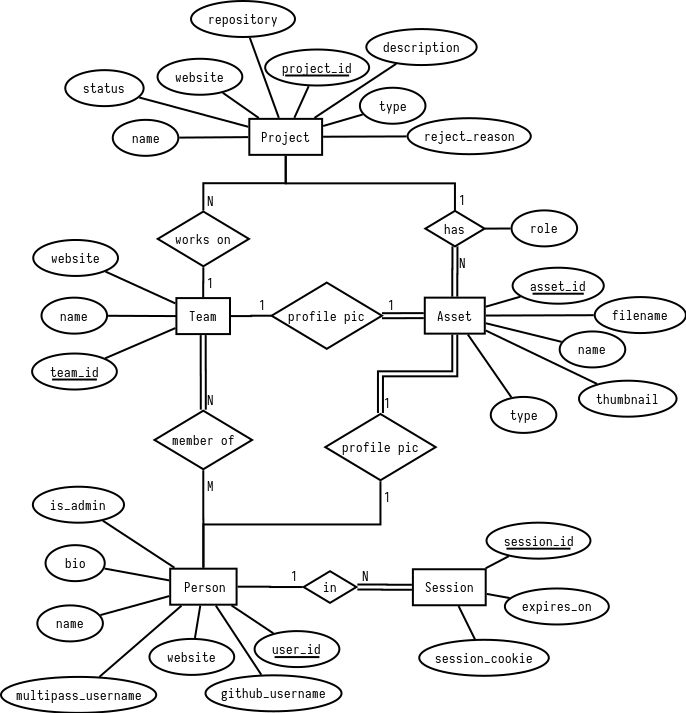
\includegraphics[width=\textwidth]{erd-new}
    \caption{The ERD for \app}
    \label{fig:erd}
\end{figure}

\subsection{Schema Explanation}
% - A section describing your dataset(s)
%
%     - What is interesting about this dataset?
%     - Where was the data obtained?
%     - What (if any) license restrictions are there on the use of the data?
%     - Describe the table or tables and significant attributes as loaded into the database.
\subsubsection{Entities}
The database contains the following entities: Projects, Teams, Assets, People,
and Sessions. The Project, Team and Person entities are self explanatory. The
Asset entity represents a single uploaded asset. These assets could be profile
pictures or project assets. Project assets can be any type of file such as
program executables, videos, or source code to name a few. The Session entity
represents a user session and associates a user of \app in their browser with
their user account in the database.

\subsubsection{Relationship}
People (users) can be in multiple Sessions. This relationship links browser
sessions with users in the database. People can be members of as many of teams
as they would like and teams may have multiple team members (m-n relationship).
Teams can work on multiple projects, but only one team can work on any given
project (1-n relationship). Each Project can have multiple assets and each asset
associated with a project has a role which could be anything from “project
executable” to “readme file”. Additionally, every user and team can have a
single profile picture asset. Assets can have at most one owner which can be
either a person, team, or project.

The reasons for most of the relationships are fairly intuitive, but we made a
few interesting design decisions. First, all assets are stored in the same
table. We chose this design because we wanted to have a single registry of files
in the system rather than having multiple places that we need to manage files. A
second interesting design choice was to add a role to the Project-has-Asset
relationship. We chose to do this because in the future, we want to store
project metadata such as configuration files or Dockerfiles in the system for
when we display the project on the ACM TV.

It would be better if each asset has a reference to one, and only one, owner
(which is either a person, project, or team). Then the role of that asset
(profile pic, readme, slide, etc.) determines its actual role. Getting a profile
pic would then be done using the query

\begin{minted}{postgresql}
    SELECT * FROM assets WHERE owner=person_id AND role=`profile_pic'
\end{minted}

rather than

\begin{minted}{postgresql}
SELECT * FROM people AS p JOIN assets AS a ON a.id=p.profile_pic WHERE p.id=person
\end{minted}

Unfortunately, this relationship is not easy to represent
in SQLAlchemy and as we were developing the models for the application we did
not fully understand the framework and we haven't gotten around to fixing it.

\section{Application Implementation}
% - A section describing the awesome cool thing you did with your data. This
%   might include charts and data visualizations, screen captures of software,
%   interesting queries, and text descriptions.

\subsection{Authentication and Authorization}
All actions that require authentication perform a lookup of the session id
cookie in the Session table to determine if the user is logged in. We then use
the user to determine what projects and teams the user has permission to edit.

\subsection{Application Structure}
We used an Model-View-Controller (MVC) architectural pattern for our
application. This pattern is very common among modern web applications and was
especially suited for our application.

\subsubsection{Model}
The models in our application are essentially wrappers around the SQL entities
in the database. To communicate with the database we used SQLAlchemy, an Object
Relational Mapping (ORM) tool that can build and manipulate databases. The
primary use of the database was to aggregate projects and project information,
which would then be forwarded onto the ACM TV after approval. One of the major
design decisions made was to store the data for the project assets on the file
system of the server and only keep basic information about the asset, such as
the asset name, in the SQL database. The model logic handled the linkage between
the filesystem and the database. This allowed for the database to be
significantly lighter, and also allowed us to circumvent some restrictions that
that SQL databases have with directly storing files, such as size limits. This
can also give a performance increase by reducing the number of copies necessary
to serve an asset (Bottle can stream directly from disk rather than copying
through the ORM).

\subsubsection{View}
We chose to try and minimize the amount of JavaScript required in our
application. To accomplish this, we tried to maximize the amount of HTML
dynamically generated on the server. This required a templating engine and we
chose to use Kajiki. Kajiki dynamically generates HTML using data from the
application including directly from our SQL database. This is done through
template files which are largely pure XHTML, but can include Python within the
XHTML elements attributes. This embedded Python can filter, repeat, and alter
its associated HTML elements. One advantage of this method is that we were able
to generate large and complex XHTML without much code overhead.

\subsubsection{Controller}
We used Bottle to route HTTP requests to the corresponding controllers. Bottle
is a fast, simple and lightweight WSGI micro web-framework for Python and is the
driving force of our application. When an HTTP request comes into the server,
Bottle calls the corresponding Python function to construct a response to return
to the user. Bottle allows us to determine what web page needs to be served to a
user, grabs the necessary database information from the SQLAlchemy models, and
then passes the information to Kajiki to interact with the user. This library is
the glue that connects all of the pieces together.

\subsection{Additional Libraries}
In addition to the Python libraries mentioned above, we used a few libraries to
build the UI. The primary libraries that we used were Bootstrap, jQuery, and
Compass. Bootstrap provides a large variety of nice styles for HTML components
and provides some convenient JavaScript utilities. jQuery gives us convenient
DOM manipulation abstractions in JavaScript. We used Compass, a CSS compiler,
which provides some nice features such as file importing and easy minification
of the resulting CSS.

\section{Implementation Difficulties}
% - A section describing the technical challenges you dealt with in obtaining,
%   manipulating, and loading the dataset(s).
Making sure asset information stayed consistent between different parts of the
ORM and the SQL database proved to be a challenging task. While the ORM easily
sets up and builds the necessary SQL tables, additional configuration is
required to ensure that calls to remove assets are propagated throughout the ORM
and the database. One specific issue that we encountered during development was
that the project object created in the ORM did not recognize when rows were
dropped from the asset and asset cross-reference table. By adding in a couple
configurations, we were able to remove assets directly from the project, which
would then drop the corresponding rows in the project-asset cross reference
table and the asset table. Once we figured out how to use this feature, the ORM
made it extremely intuitive to work with.

Another issue we ran across was the orphaning of assets in the file system.
While the internal issues between the SQL database and the ORM were solved with
some additional ORM configuration, asset data still remained on the file system
after the asset information was deleted off of the ORM and database. The
orphaning issue was solved by using the Python standard library to delete the
file data off of the file system before removing the rows off of the table.

\section{What We Learned}
None of us had used an ORM before this project. While there were a couple of
exceptions, setting up the database schema was very simple and intuitive. Each
table is simply a new Python class. Columns and relationships can be added to a
table by adding variables of type Column and Relationship, respectively.
Manipulating and querying variables was also very convenient since queries were
returned as Python objects. This allowed the SQL data to work very well with the
other Python libraries, and allowed us to pass information from queries directly
from the ORM to the XHTML templates to display user, project, and team
information.

Another valuable skill we learned was integrating a file system with the SQL
database in order to store files. With the help of the Python standard library,
storing files on disk was pretty straightforward. After we retrieved the file
using Bottle, we took the file information (such as the file name) and added it
to the asset table on the SQL server. The file data was then assigned a UUID and
stored on the file system. Whenever we needed to serve a file, we would use
Bottle to take the data off of the disk, and then attach the name of the file
from the SQL server onto the data before serving it to the user.

We also learned a great deal about web application design. Although we were
familiar with the MVC paradigm, we had never implemented a full MVC app before.
Additionally, we used a variety of libraries that we had never used before or
had had minimal experience with. Although none of the libraries had an
especially steep learning curve, learning all of the libraries at the same time
was not trivial.

\section{Conclusion}
Through the process of building this app, we learned about the application
development process

\end{document}
